\chapter{A Visual Language for the Whole Paper}

Maya Song, a doctoral candidate in oceanography, is preparing the final manuscript of a synthesis paper before submission. Drawing on four public observational and global carbon-budget datasets, the paper reviews how the global ocean absorbs the vast majority of excess heat in the climate system alongside roughly a quarter of anthropogenic carbon dioxide ($\text{CO}_2$) emissions. The manuscript contains four figures: Figure 1 is a conceptual schematic of the main pathways of air--sea heat and anthropogenic carbon uptake; Figure 2 presents long-term records of atmospheric $\text{CO}_2$ dry-air mole fraction at Mauna Loa Observatory, Hawaii, together with surface seawater partial pressure of $\text{CO}_2$ ($p\text{CO}_2$) and pH at Station ALOHA in the subtropical North Pacific; Figure 3 shows pentadal global ocean heat content anomalies in the $0\text{--}700\ \text{m}$ and $0\text{--}2000\ \text{m}$ layers; and Figure 4 tracks global anthropogenic $\text{CO}_2$ emissions and their partitioning among atmospheric growth, the ocean sink, and the land sink, paired with the ocean sink's share of total emissions.

Maya created these four figures over two months in separate work sessions: Figure 1 with an image generation tool, and Figures 2 through 4 on different days using separate scripts and conversational sessions. Viewed one at a time on a laptop screen, each plot looked passable. Just before submission, however, her advisor asked her to print all four figures side by side on a single A4 sheet (Figure~\ref{fig:ch04-01}). Seen together, the set fell apart at once---anticipating the exact critique a reviewer would later write: ``The figures are difficult to compare across the paper; colour assignments and symbol meanings contradict one another from one figure to the next.''

\begin{figure}[htbp]\centering
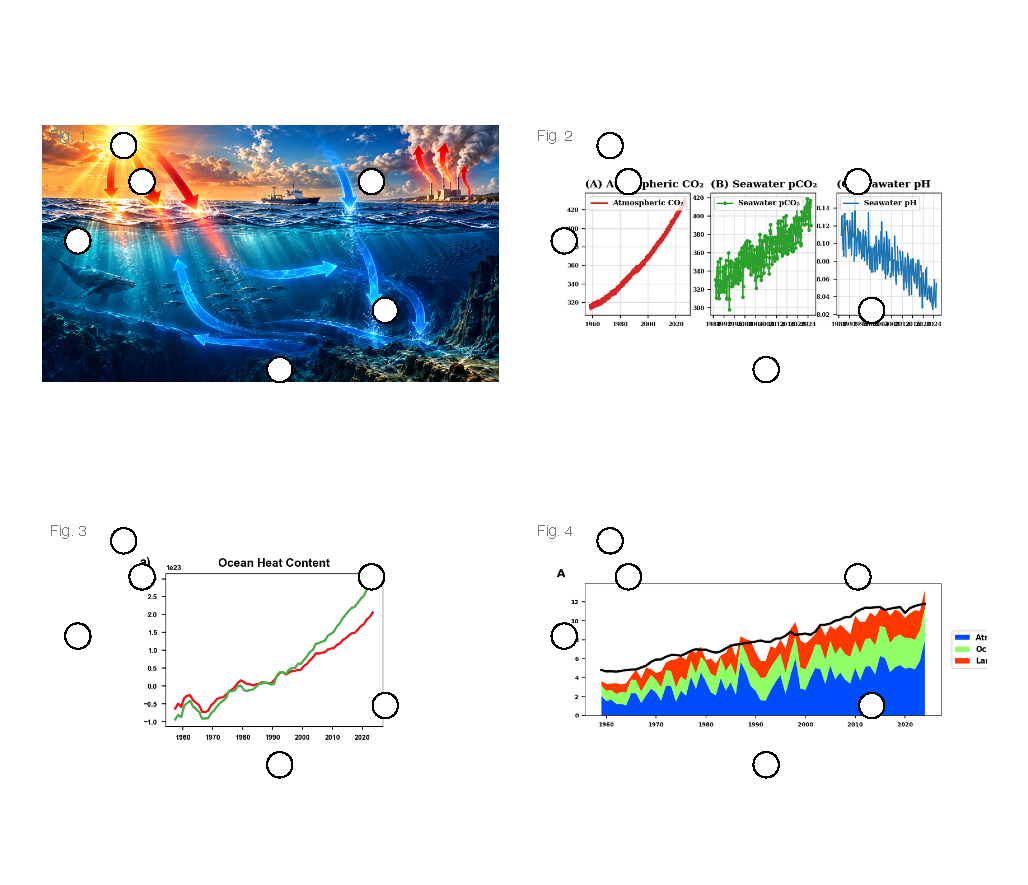
\includegraphics[width=\linewidth]{figures/ch04/ch04-01-inconsistent-set-en.pdf}
\caption{Four figures that each look acceptable in isolation but fail to work as a set (a deliberately inconsistent example). Six classes of conflict appear across the page: (1) red denotes solar radiation and smokestack emissions in Fig.\ 1, atmospheric $\text{CO}_2$ in Fig.\ 2, $0\text{--}700\ \text{m}$ ocean heat content in Fig.\ 3, and the land carbon sink in Fig.\ 4; (2) arrows of a single colour stand for unrelated processes in the schematic; (3) Fig.\ 3 relies solely on red versus green to separate two curves and omits a legend; (4) Fig.\ 4 uses a rainbow colormap for stacked areas while its legend box is clipped off the right edge; (5) the four figures mix three typefaces and four panel-labelling styles, and unconfigured Unicode characters produce missing-glyph boxes inside the callout circles and subplot titles; (6) the glossy 3D schematic introduces unmentioned decorative objects including a sun, a ship, a whale, and schools of fish. Figs.\ 2--4 plot real public data; only the styling differs.}\label{fig:ch04-01}
\end{figure}

Scanning across the four quadrants of Figure~\ref{fig:ch04-01} shows why an inconsistent figure set slows comprehension. In the top-left quadrant (Fig.\ 1), glowing red 3D arrows both shoot downward from the sun into the sea (solar heating) and rise from factory smokestacks into the sky (anthropogenic carbon emissions). In the top-right quadrant (Fig.\ 2a), a thick red curve denotes atmospheric $\text{CO}_2$. In the bottom-left quadrant (Fig.\ 3), the red curve switches meaning to $0\text{--}700\ \text{m}$ ocean heat content. In the bottom-right quadrant (Fig.\ 4), the red top band of the stacked area plot denotes the land carbon sink. Green shifts from surface seawater $p\text{CO}_2$ (Fig.\ 2b) to $0\text{--}2000\ \text{m}$ heat content (Fig.\ 3) to the ocean carbon sink (Fig.\ 4), while blue jumps from air--sea gas exchange and deep circulation arrows (Fig.\ 1) to seawater pH (Fig.\ 2c) to atmospheric $\text{CO}_2$ growth (Fig.\ 4). At each figure transition, the reader must unlearn the previous colour code and hunt for a legend to decode the new plot (Table~\ref{tab:ch04-diag}).

\begin{table}[htbp]\centering\footnotesize
\setlength{\tabcolsep}{3pt}
\renewcommand{\arraystretch}{1.15}
\caption{Diagnosis of the visual conflicts in the inconsistent first draft (Figure~\ref{fig:ch04-01}) and the cognitive cost imposed on the reader.}\label{tab:ch04-diag}
\begin{tabularx}{\linewidth}{@{}Y>{\raggedright\arraybackslash}p{18mm}Y@{}}
\toprule
\textbf{Visual conflict in the first draft} & \textbf{Location} & \textbf{Cognitive cost to the reader} \\
\midrule
Red, green, and blue switch meaning across figures (red denotes heat and emissions in Fig.\ 1, atmospheric $\text{CO}_2$ in Fig.\ 2, upper-ocean heat in Fig.\ 3, and the land sink in Fig.\ 4) & Figs.\ 1--4 & Readers cross-referencing panels mistakenly equate matching colours with the same physical quantity or carbon reservoir \\
Blue arrows represent both water circulation and air--sea carbon exchange; red arrows represent both solar heating and smokestack carbon emissions & Fig.\ 1 & Readers cannot tell from an arrow's geometry or hue which physical or biogeochemical process is depicted \\
Two curves of equal stroke width are distinguished solely by pure red versus pure green, with neither a legend nor direct labels & Fig.\ 3 & Readers with red--green colour vision deficiency cannot tell the $0\text{--}700\ \text{m}$ and $0\text{--}2000\ \text{m}$ layers apart \\
A \texttt{jet} rainbow stacked area plot represents the three carbon sinks, and omitting the budget imbalance causes the stacked top edge to cross above the black total-emissions line & Fig.\ 4 & The colour order has no physical meaning, sharp luminance jumps create false boundaries, and the sum of sinks appears to exceed total emissions \\
Three typefaces and four panel-label formats (\texttt{(A)}, \texttt{a)}, \texttt{A}, and none) are mixed, while Unicode subscripts and circled numbers render as missing-glyph boxes & Figs.\ 1--4 & The manuscript looks cobbled together; text references such as ``Fig.\ 3a'' or ``Fig.\ 2b'' are slow to locate \\
Type sizes range from $6\ \text{pt}$ to $12\ \text{pt}$, in-figure titles duplicate the captions, and the right-hand legend box is sliced off by the canvas edge & Figs.\ 2--4 & Visual hierarchy breaks down, plot area is wasted on redundant headers, and truncated labels (\texttt{Atr...}, \texttt{Oc...}, \texttt{La...}) leave series unidentified \\
A glossy 3D schematic clashes with flat 2D data plots and introduces a sun, a ship, a whale, and schools of fish & Fig.\ 1 & Unmentioned processes (solar radiation optics, shipboard surveys, marine food webs) distract from the paper's scope \\
Vertical-axis unit conventions vary, and multiplying values already in $10^{22}\ \text{J}$ by $10^{22}$ triggers a stray ``\texttt{1e23}'' offset label with no unit name & Figs.\ 2--4 & Readers must pause to reconcile orders of magnitude and infer missing physical dimensions \\
\bottomrule
\end{tabularx}
\end{table}

The figures in a paper are not standalone illustrations; they form a coordinated visual argument. Whenever multiple panels revisit the same physical quantities or reservoirs, choices of colour, typography, line weight, arrow geometry, and icon style constitute a paper-wide \textbf{visual language}. This chapter shows how to write a one-page visual specification before generating final figures, translate its clauses into style blocks for \scidraw{}, and audit every output so that all figures speak the same language.

\section{Colour Carries Meaning First}

When researchers choose colours for a figure, their first instinct is often aesthetic: picking a palette that looks pleasing on screen. In scientific figures, however, the primary role of colour is not decoration but \textbf{semantic encoding}. Readers automatically assume that a recurring, salient hue refers to the same variable or reservoir across a paper (Wong, 2010; Krzywinski, 2013). When colours are assigned ad hoc from default software cycles in separate sessions, cross-figure reasoning breaks down.

\textbf{First, assign semantic colours by scientific meaning and lock them across the manuscript.} Building a visual language starts with listing every core quantity or reservoir that recurs across your figures, assigning each role a dedicated hexadecimal colour (a semantic colour), and stating both what it \textit{is used for} and what it \textit{must never be used for}. In Maya's paper, the specification locks six quantitative roles and one schematic-only role:
\begin{itemize}
\item \textbf{Atmospheric carbon ($\text{CO}_2$):} Orange (\texttt{\#E69F00}), used for atmospheric $\text{CO}_2$ dots in Fig.\ 1, the Mauna Loa $\text{CO}_2$ curves in Fig.\ 2a, and atmospheric carbon growth in Fig.\ 4a. Never used for heat or oceanic variables.
\item \textbf{Ocean carbon:} Blue (\texttt{\#0072B2}), used for surface seawater dissolved inorganic carbon (DIC) in Fig.\ 1, seawater $p\text{CO}_2$ in Fig.\ 2b, the ocean carbon sink in Fig.\ 4a, and the ocean sink share in Fig.\ 4b. Never used for background water or heat.
\item \textbf{Land carbon:} Bluish green (\texttt{\#009E73}), reserved exclusively for the land carbon sink in Fig.\ 4a. Never used to colour phytoplankton icons in the schematic.
\item \textbf{Heat:} Vermilion (\texttt{\#D55E00}), used for heat-flux arrows in Fig.\ 1 and ocean heat content curves in Fig.\ 3. Never used for any carbon quantity.
\item \textbf{Seawater pH:} Reddish purple (\texttt{\#CC79A7}), dedicated solely to surface seawater pH in Fig.\ 2c.
\item \textbf{Anthropogenic emissions and carbon input fluxes:} Near-black dark gray (\texttt{\#3C3C3C}), used for total emissions in Fig.\ 4a and straight carbon-flux arrows in Fig.\ 1.
\item \textbf{Water-mass transport (schematic only):} Sky blue (\texttt{\#56B4E9}) as a broad semi-transparent band, reserved in Fig.\ 1 for sinking and interior water circulation; never used for data curves.
\end{itemize}

\textbf{Second, cap the number of semantic hues and separate variants of a single quantity using lightness tints of the same hue.} Visual working memory holds at most six or seven distinct colour categories without repeated trips back to a key (Wong, 2010). All structural elements---axes, reference lines, background zones, and icon bodies---must recede into neutral grays (\texttt{\#F2F2F2}, \texttt{\#BDBDBD}, \texttt{\#7A7A7A}). When a single panel compares two variants of the same physical quantity---such as $0\text{--}700\ \text{m}$ and $0\text{--}2000\ \text{m}$ ocean heat content anomalies in Fig.\ 3---do not borrow green or blue from the carbon budget. Instead, \textbf{keep the hue locked to vermilion for heat and separate depth layers by lightness}: plot $0\text{--}2000\ \text{m}$ in full-strength vermilion (\texttt{\#D55E00}) and $0\text{--}700\ \text{m}$ in a $55\%$ tint mixed $45\%$ toward white, labelling each curve directly at its right end (Figure~\ref{fig:ch04-02}, Figure~\ref{fig:ch04-03}). The reader sees immediately both that Fig.\ 3 represents ocean heat and which curve belongs to which depth layer.

\begin{figure}[htbp]\centering
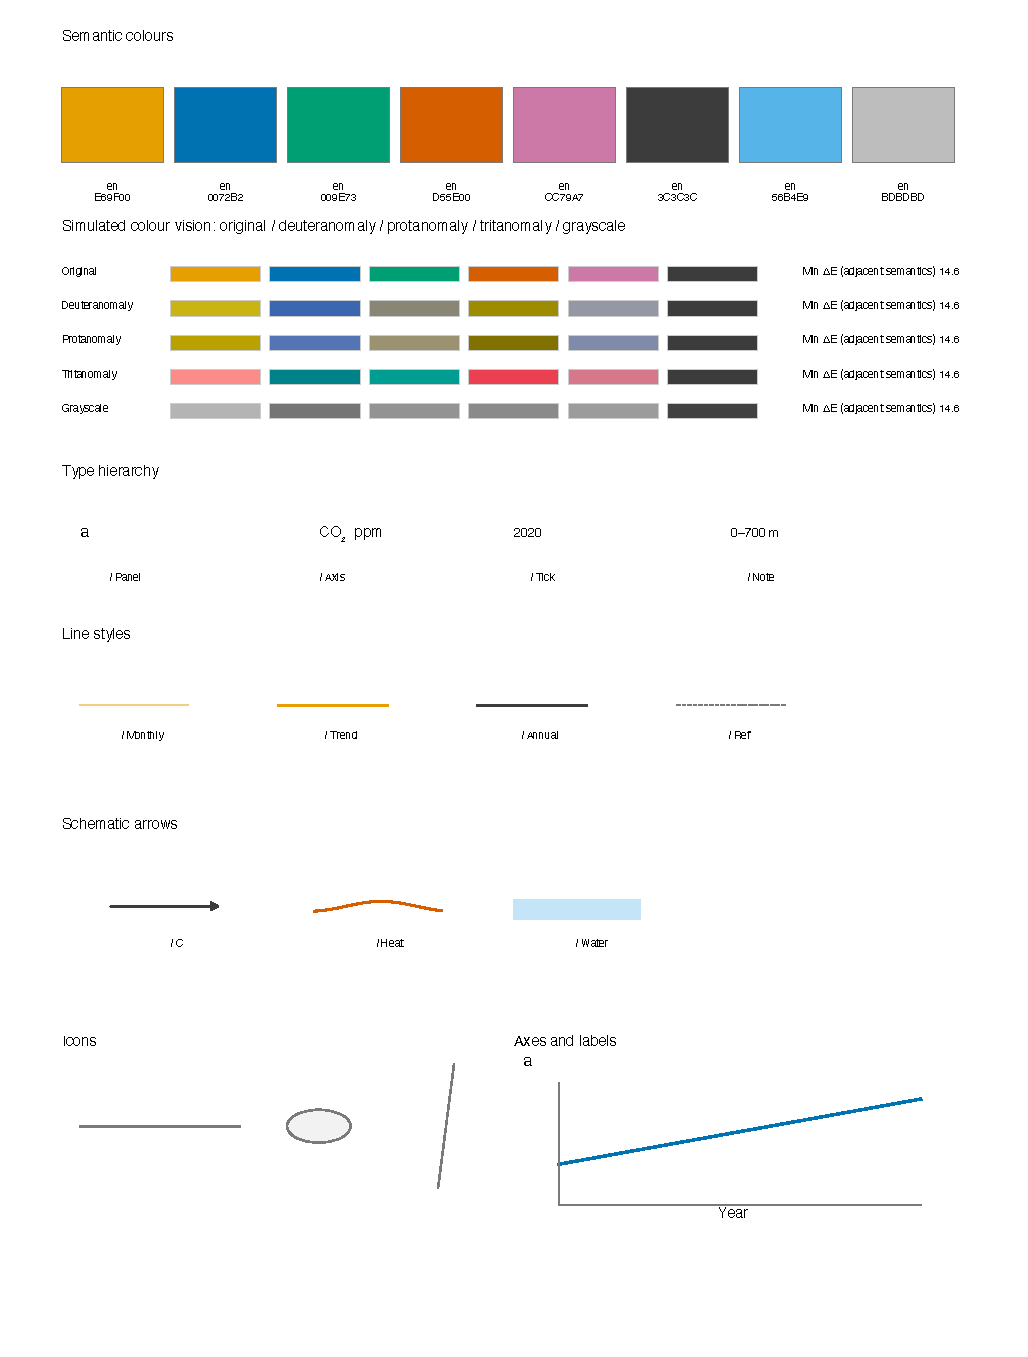
\includegraphics[width=0.95\linewidth,height=0.80\textheight,keepaspectratio]{figures/ch04/ch04-02-spec-page-en.pdf}
\caption{A one-page visual specification (v1) for the case-study manuscript. From top to bottom, the sheet defines semantic colour swatches, colour-vision deficiency (CVD) simulations and grayscale lightness strip, four-level type hierarchy at final print size, data-figure line styles, schematic process arrows, neutral icon style, and axis layout. The value at the right of each simulation row ($14.6$) is the smallest perceptual colour difference (CAM02-UCS $\Delta E$) between semantic colours that appear side by side in the same panel, computed by the script.}\label{fig:ch04-02}
\end{figure}

\textbf{Third, start from a colour-vision-accessible palette and never rely on red versus green alone.} Roughly $8\%$ of men of Northern European descent experience congenital red--green colour vision deficiency, most commonly deuteranomaly (Wong, 2011; note that a 2023 Author Correction to this article revised the cone sensitivity labels and terminology in the original figure). In the inconsistent draft of Fig.\ 3 (Figure~\ref{fig:ch04-01}), the two depth layers were plotted as equal-width lines in saturated red (\texttt{\#E41A1C}) and green (\texttt{\#4DAF4A}). Under simulated deuteranomaly (Figure~\ref{fig:ch04-03}, top right), those two curves collapse into nearly indistinguishable olive-brown lines. Begin instead from a colour-vision-accessible palette such as Okabe--Ito (Okabe and Ito, 2008; Wong, 2011) or ColorBrewer (Brewer).

\begin{figure}[htbp]\centering
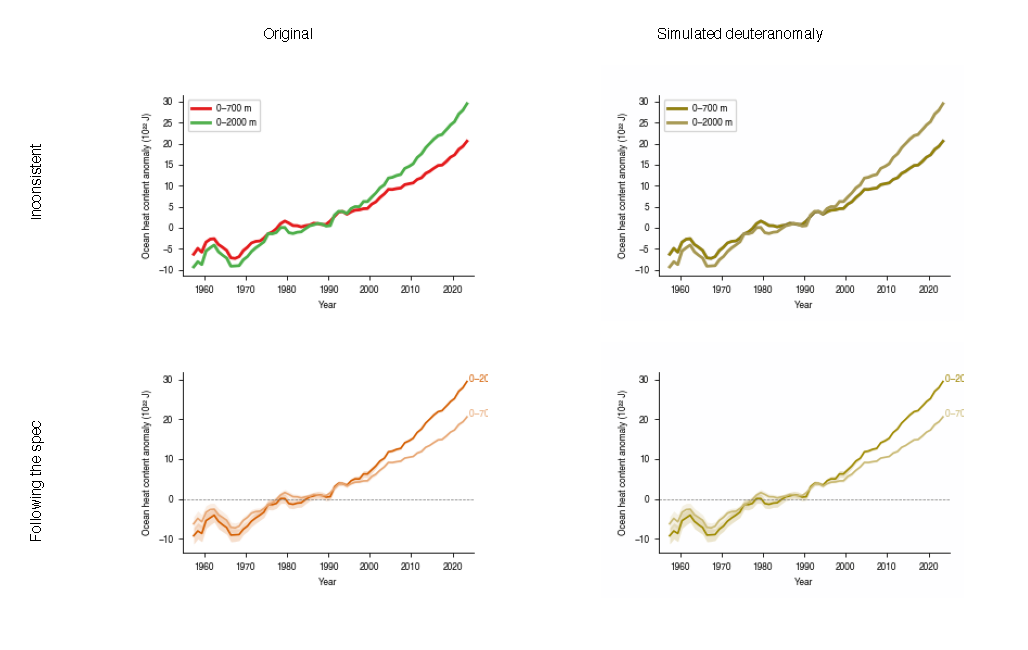
\includegraphics[width=\linewidth]{figures/ch04/ch04-03-cvd-check-en.pdf}
\caption{Two curves distinguished only by red and green become hard to tell apart under simulated deuteranomaly (top row); two lightnesses of one semantic hue paired with uncertainty bands and direct labels remain clearly separable (bottom row). The right column applies a full-image pixel simulation of deuteranomaly at severity $100$ using \texttt{colorspacious}. Data: NOAA NCEI pentadal global ocean heat content anomaly (Levitus et al., 2012).}\label{fig:ch04-03}
\end{figure}

\textbf{Fourth, combine colour-vision simulation and grayscale checks with redundant encoding.} Even an accessible palette needs quantitative verification when multiple curves share a panel. The second band of Figure~\ref{fig:ch04-02} simulates all eight swatches under deuteranomaly, protanomaly, and tritanomaly (at severity $100$ in \texttt{colorspacious}) and CIELAB lightness grayscale ($L^*$), reporting the minimum CAM02-UCS colour difference $\Delta E$ between semantic colours that appear side by side in the same panel. As a practical self-check guideline---offered here as an operational rule of thumb rather than a formal standard---\textbf{adjacent series in the same panel should maintain a CAM02-UCS distance of $\Delta E \ge 15$ under CVD simulation and a grayscale lightness difference of $\Delta L^* \ge 15$; whenever a pair falls near or below that threshold, add redundant encoding via line style, marker shape, or direct end-of-line labels.}

In Figure~\ref{fig:ch04-02}, the minimum adjacent distance across the simulation rows is $\Delta E = 14.6$---just shy of $15$---and in the grayscale row, ocean blue (\texttt{\#0072B2}), land bluish green (\texttt{\#009E73}), and heat vermilion (\texttt{\#D55E00}) sit at similar luminances. Thus no multi-hue palette can rely on hue alone. As the bottom row of Figure~\ref{fig:ch04-03} shows, pairing dark and light vermilion with $\pm 1\ \text{WOse}$ shading bands and right-end depth labels keeps the two curves distinct under severity-$100$ deuteranomaly simulation. Remember that numerical CVD simulation is only a colorimetric approximation; printing a black-and-white check sheet and asking a colleague with colour vision deficiency to review the figures remain essential before submission.

\textbf{Fifth, map continuous fields with perceptually uniform colormaps and retire rainbow colormaps.} Avoid rainbow colormaps such as \texttt{jet} when encoding continuous fields or stacked quantities. Because \texttt{jet} has a non-monotonic luminance profile, it creates false visual boundaries in cyan and yellow zones and fails under colour vision deficiency (Crameri et al., 2020). Use perceptually uniform sequential colormaps such as \texttt{viridis} or \texttt{cividis} (Nu\~nez et al., 2018) for single-ended variables, and zero-centered diverging colormaps for positive and negative anomalies.

\section{Type Hierarchy at Final Print Size}

A second source of visual incoherence in Figure~\ref{fig:ch04-01} is uncontrolled typography: Fig.\ 2 uses \texttt{DejaVu Serif} ($11\ \text{pt}$) with labels ``\texttt{(A)(B)(C)}''; Fig.\ 3 uses bold \texttt{Arial} ($9\ \text{pt}$) with ``\texttt{a)}''; and Fig.\ 4 uses \texttt{DejaVu Sans} ($8\ \text{pt}$) with ``\texttt{A}''. Because each plot was drawn on a different canvas size and scaled to fit the page, effective font sizes vary erratically across panels.

\textbf{First, lock the target journal's final print width before setting font sizes.} If you plot on a default $10 \times 6\ \text{inch}$ ($254 \times 152\ \text{mm}$) canvas and later shrink the figure into an $85\ \text{mm}$ single column, every font shrinks to one-third of its nominal size, turning a $10\ \text{pt}$ tick label into an illegible $3.3\ \text{pt}$ (Rougier et al., 2014; Wong, 2011 Typography). Always set physical canvas widths from the target journal's author instructions first---typically $85\text{--}89\ \text{mm}$ for single-column figures and $174\text{--}183\ \text{mm}$ for double-column figures ($174\ \text{mm}$ for Figs.\ 1, 2, and 4; $85\ \text{mm}$ for Fig.\ 3 in our case study)---specify font sizes in points at that exact width, and inspect the exported PDF at $100\%$ print scale.

\textbf{Second, establish a four-level type hierarchy in a single sans-serif family.} Govern all text across the manuscript with four levels (Figure~\ref{fig:ch04-02}, ``Type hierarchy''):
\begin{enumerate}
\item \textbf{Panel letters ($8\ \text{pt}$ bold):} Lowercase bold \textbf{a}, \textbf{b}, \textbf{c} without parentheses, placed outside the top-left corner of the axes frame.
\item \textbf{Axis labels ($7\ \text{pt}$ regular):} ``Quantity name (unit)'', such as ``Atmospheric $\text{CO}_2$ (ppm)''.
\item \textbf{Tick labels ($6\ \text{pt}$ regular):} Horizontal, unrotated, and non-overlapping.
\item \textbf{In-figure annotations and schematic labels ($6\text{--}7\ \text{pt}$ regular):} Direct curve labels and brief notes use $6\ \text{pt}$ regular (curve labels match the series colour); schematic region/object labels use $7\ \text{pt}$ and process labels use $6\ \text{pt}$.
\end{enumerate}

Use one sans-serif typeface (\texttt{Helvetica}, \texttt{Arial}, or \texttt{TeX Gyre Heros}) across all figures so small $6\text{--}7\ \text{pt}$ labels remain crisp (Wong, 2011 Typography). When producing bilingual editions, pair a uniform-stroke CJK gothic font (such as \texttt{FandolHei} or Source Han Sans) at the same point sizes while keeping numerals and units in the Latin sans-serif font.

Inspecting our rendered figures at $200\%$ zoom highlights a pervasive font-encoding trap. Look at the callout circles and Fig.\ 2 titles in Figure~\ref{fig:ch04-01}, the sample rows in Figure~\ref{fig:ch04-02}, and the vertical axis labels of Figure~\ref{fig:ch04-05} and Figure~\ref{fig:ch04-07}. When a script passes raw Unicode subscripts (such as the subscript $2$ in $\text{CO}_2$), Unicode superscript minus signs (in $\text{GtC yr}^{-1}$), circled numbers, or bilingual CJK strings directly to a font that lacks those glyphs, two failures occur: in raster or unconfigured font backends, missing characters render as empty missing-glyph boxes---visible inside the callout circles and Fig.\ 2 titles of Figure~\ref{fig:ch04-01} and the bilingual sample strings of Figure~\ref{fig:ch04-02} (such as ``\texttt{CO [box]ppm[box]}''); in vector PDF backends, missing glyphs can be silently dropped without warning---turning ``Atmospheric $\text{CO}_2$ (ppm)'' and ``Seawater $p\text{CO}_2$ ($\mu\text{atm}$)'' into ``Atmospheric CO (ppm)'' and ``Seawater pCO ($\mu$atm)'' in Figure~\ref{fig:ch04-05}, and turning ``$\text{GtC yr}^{-1}$'' into ``$\text{GtC yr}^{1}$'' in Figure~\ref{fig:ch04-07}. Meanwhile, a tuple-indexing bug in the specification script printed the language code ``\texttt{en}'' above each hex value in Figure~\ref{fig:ch04-02}. Never trust automatic font fallback for subscripts or exponents; use explicit math-mode or markup syntax (such as \texttt{\textbackslash textsubscript\{2\}} and \texttt{\$yr\^{}\{-1\}\$}) and check every exported PDF at $200\%$ zoom.

\textbf{Third, standardize unit notation, replace boxed legends with direct labels, and remove in-figure titles.} In Fig.\ 3 of Figure~\ref{fig:ch04-01}, multiplying values already reported in $10^{22}\ \text{J}$ by $10^{22}$ triggered a stray ``\texttt{1e23}'' offset label with no unit name. Our specification standardizes units into parenthetical SI form ($10^{22}\ \text{J}$, $\text{GtC yr}^{-1}$, $\mu\text{atm}$, ppm), deletes subplot titles that duplicate the caption, and replaces legend boxes with colour-matched labels at the right ends of the curves (Wong, 2011 Typography).

\section{One Meaning per Line and Arrow}

In the inconsistent draft (Figure~\ref{fig:ch04-01}), geometric primitives are equally muddled: Fig.\ 2a plots monthly means and deseasonalized trends as two heavy $2\ \text{pt}$ red curves on top of each other; Fig.\ 2b connects discrete cruise samples with straight green line segments; and Fig.\ 1 uses identical glowing arrows for gas exchange, solar heating, and ocean circulation. The core rule is straightforward: \textbf{one visual form per meaning, and one meaning per visual form.}

In data figures, series with different statistical meanings or sampling frequencies are separated by stroke weight, tint, marker geometry, and opacity (Table~\ref{tab:ch04-lines}):

\begin{table}[htbp]\centering\footnotesize
\setlength{\tabcolsep}{4pt}
\renewcommand{\arraystretch}{1.15}
\caption{Line, marker, and shading rules for the case-study data figures (Section C of the visual specification).}\label{tab:ch04-lines}
\begin{tabularx}{\linewidth}{@{}>{\raggedright\arraybackslash}p{36mm}Y>{\raggedright\arraybackslash}p{42mm}@{}}
\toprule
\textbf{Statistical nature of series} & \textbf{Specified visual encoding} & \textbf{Application in the case study} \\
\midrule
High-frequency raw observations (monthly means) & $0.5\ \text{pt}$ thin solid line in a $50\%$ lighter tint of the series semantic colour & Fig.\ 2a Mauna Loa monthly mean atmospheric $\text{CO}_2$ \\
Deseasonalized or running-mean trend & $1.2\ \text{pt}$ thick solid line in full-strength semantic colour & Fig.\ 2a deseasonalized $\text{CO}_2$, Fig.\ 3 pentadal heat content, Fig.\ 4b 10-year running mean \\
Discrete shipboard cruises or irregular sampling & Solid circular dots ($2.5\ \text{pt}$ diameter) with \textbf{no connecting line} & Fig.\ 2b surface seawater $p\text{CO}_2$, Fig.\ 2c surface pH, Fig.\ 4b annual sink share \\
Annual budget time series & $1.0\ \text{pt}$ solid line in the corresponding semantic colour & Fig.\ 4a annual emissions and the three carbon sinks \\
Uncertainty intervals (standard error or mean uncertainty) & $20\%$ opacity filled band in the series semantic colour, with no border line & Fig.\ 3 ($\pm 1\ \text{WOse}$ pentadal standard error), Fig.\ 4a (mean sink uncertainty bands) \\
Reference lines and station-change markers & $0.5\ \text{pt}$ dashed medium-dark gray (\texttt{\#7A7A7A}) line with $6\ \text{pt}$ gray text note & Fig.\ 2a Maunakea eruption relocation line, Fig.\ 3 zero-anomaly baseline \\
\bottomrule
\end{tabularx}
\end{table}

For example, Mauna Loa monthly means summarize continuous daily measurements, so plotting them as a $0.5\ \text{pt}$ light-orange line beneath a $1.2\ \text{pt}$ full-orange deseasonalized curve preserves the seasonal cycle while highlighting the long-term trend. Station ALOHA measurements, by contrast, come from discrete research cruises with irregular spacing and occasional gaps; connecting them with straight lines falsely implies linear interpolation between voyages, so they must be plotted as unlinked dots.

In the conceptual schematic (Fig.\ 1), we likewise assign four mutually exclusive arrow geometries to the four physical and biogeochemical processes (Table~\ref{tab:ch04-arrows}):

\begin{table}[htbp]\centering\footnotesize
\setlength{\tabcolsep}{4pt}
\renewcommand{\arraystretch}{1.15}
\caption{Process arrow rules for the case-study schematic (Section D of the visual specification).}\label{tab:ch04-arrows}
\begin{tabularx}{\linewidth}{@{}>{\raggedright\arraybackslash}p{36mm}Y>{\raggedright\arraybackslash}p{44mm}@{}}
\toprule
\textbf{Physical or biogeochemical process} & \textbf{Specified geometry and colour} & \textbf{Dual redundancy of shape and colour} \\
\midrule
Carbon fluxes (anthropogenic emissions and air--sea gas exchange) & Straight shaft, filled triangular head, near-black dark gray (\texttt{\#3C3C3C}), $1.0\ \text{pt}$ & Separated from heat flux both by hue (dark gray vs.\ vermilion) and by geometry (straight filled triangle vs.\ wavy open V) \\
Heat flux (air--sea heat uptake and downward penetration) & Sine-wave shaft, open V-shaped head, vermilion (\texttt{\#D55E00}), $1.0\ \text{pt}$ & Uses the heat-transfer wavy-arrow convention so thermal fluxes remain recognizable in grayscale or under CVD \\
Water-mass subduction and interior circulation & Broad $4\text{--}6\ \text{pt}$ semi-transparent sky-blue (\texttt{\#56B4E9}) band containing flow-aligned chevrons & Uses an areal ribbon for bulk water-mass transport, visually distinct from thin interface-flux arrows \\
Sinking organic particles (biological pump export) & Dotted shaft, small filled triangular head, near-black dark gray (\texttt{\#3C3C3C}), $0.8\ \text{pt}$ & Dotted line evokes settling particles; thinner stroke ($0.8\ \text{pt}$) signals its secondary role relative to gas exchange \\
\bottomrule
\end{tabularx}
\end{table}

Defining each arrow once in the bottom legend strip ensures that straight, wavy, ribbon, and dotted arrows never collide in meaning, even in grayscale print.

\section{Icon and Element Style}

In papers that combine schematics with data plots, a common flaw is pairing flat 2D graphs with a glossy 3D schematic full of lens flares, water caustics, and perspective shadows (Figure~\ref{fig:ch04-04}, left). Bringing the schematic into the paper's visual language requires five rules (Section E of the specification):

\textbf{First, fill icon bodies with neutral grays and reserve semantic colours strictly for tracked quantities.} Factory smokestacks and phytoplankton cells are process carriers, not plotted data variables. Colouring phytoplankton green would falsely link them to the land carbon sink (\texttt{\#009E73}) in Fig.\ 4. All icon bodies therefore use neutral gray fills (\texttt{\#F2F2F2}, \texttt{\#BDBDBD}), reserving orange for atmospheric $\text{CO}_2$ dots, blue for seawater DIC dots, vermilion for heat arrows, and sky blue for the water-transport band, while background water layers use pale desaturated blue-grays (\texttt{\#DCEBF5} for the mixed layer, \texttt{\#C9DEEE} for the interior).

\textbf{Second, align stroke weights with data-figure axes.} Because data axes use $0.6\ \text{pt}$ lines, setting icon outlines and the sea-surface wave line to $0.75\ \text{pt}$ dark gray (\texttt{\#3C3C3C}) with rounded joins unifies line weight across panels.

\textbf{Third, use flat 2D silhouettes without gradients, shadows, highlights, or photorealistic water.} A clean background keeps overlaid labels legible.

\textbf{Fourth, draw recurring features consistently across panels.} The sea-surface wave line and mixed-layer boundary keep a uniform geometry wherever they appear.

\textbf{Fifth, exclude unmentioned decorative objects and respect the scientific boundaries of the mechanism.} The left panel of Figure~\ref{fig:ch04-04} includes a blazing sun with light rays (implying shortwave radiative transfer is studied), a research ship, and model-generated whales, fish schools, and reefs---all of which misrepresent the paper's scope.

\begin{figure}[htbp]\centering
\begin{minipage}[c]{0.48\linewidth}\centering
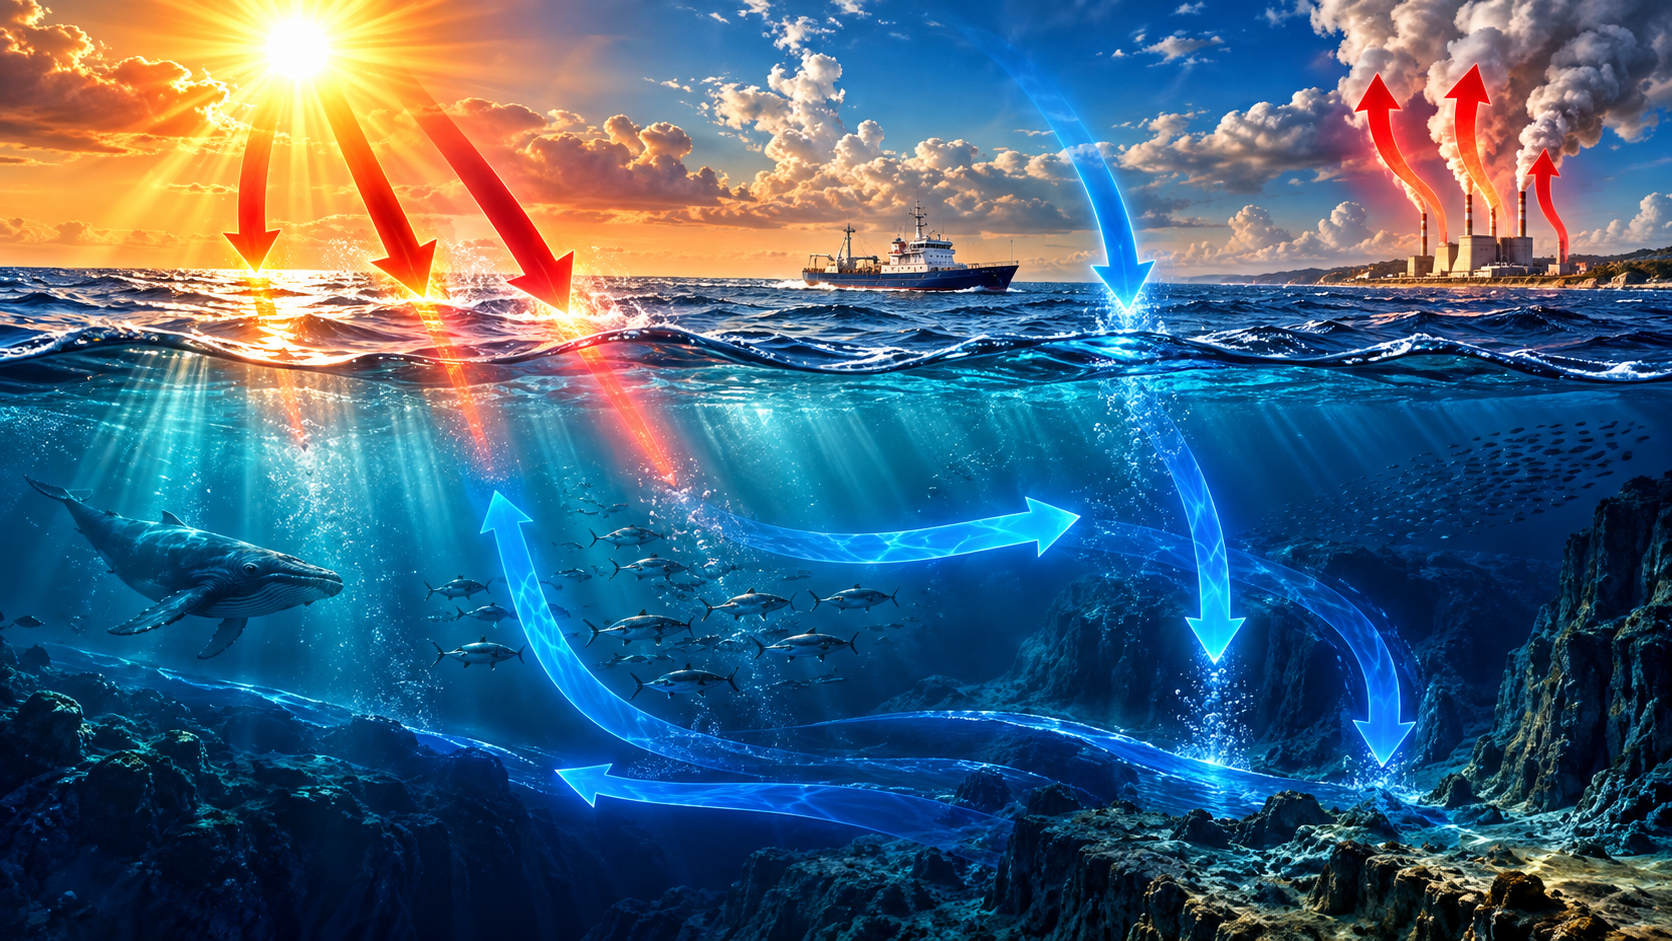
\includegraphics[width=\linewidth]{figures/ch04/ch04-04a-schematic-bad.png}
\end{minipage}\hfill
\begin{minipage}[c]{0.48\linewidth}\centering
\resizebox{\linewidth}{!}{\hbox{\setlength{\linewidth}{\textwidth}% FIG ch04-04b schematic labels (English)
\usetikzlibrary{positioning}
\begin{tikzpicture}
\node[anchor=south west,inner sep=0] (img) at (0,0) {%
  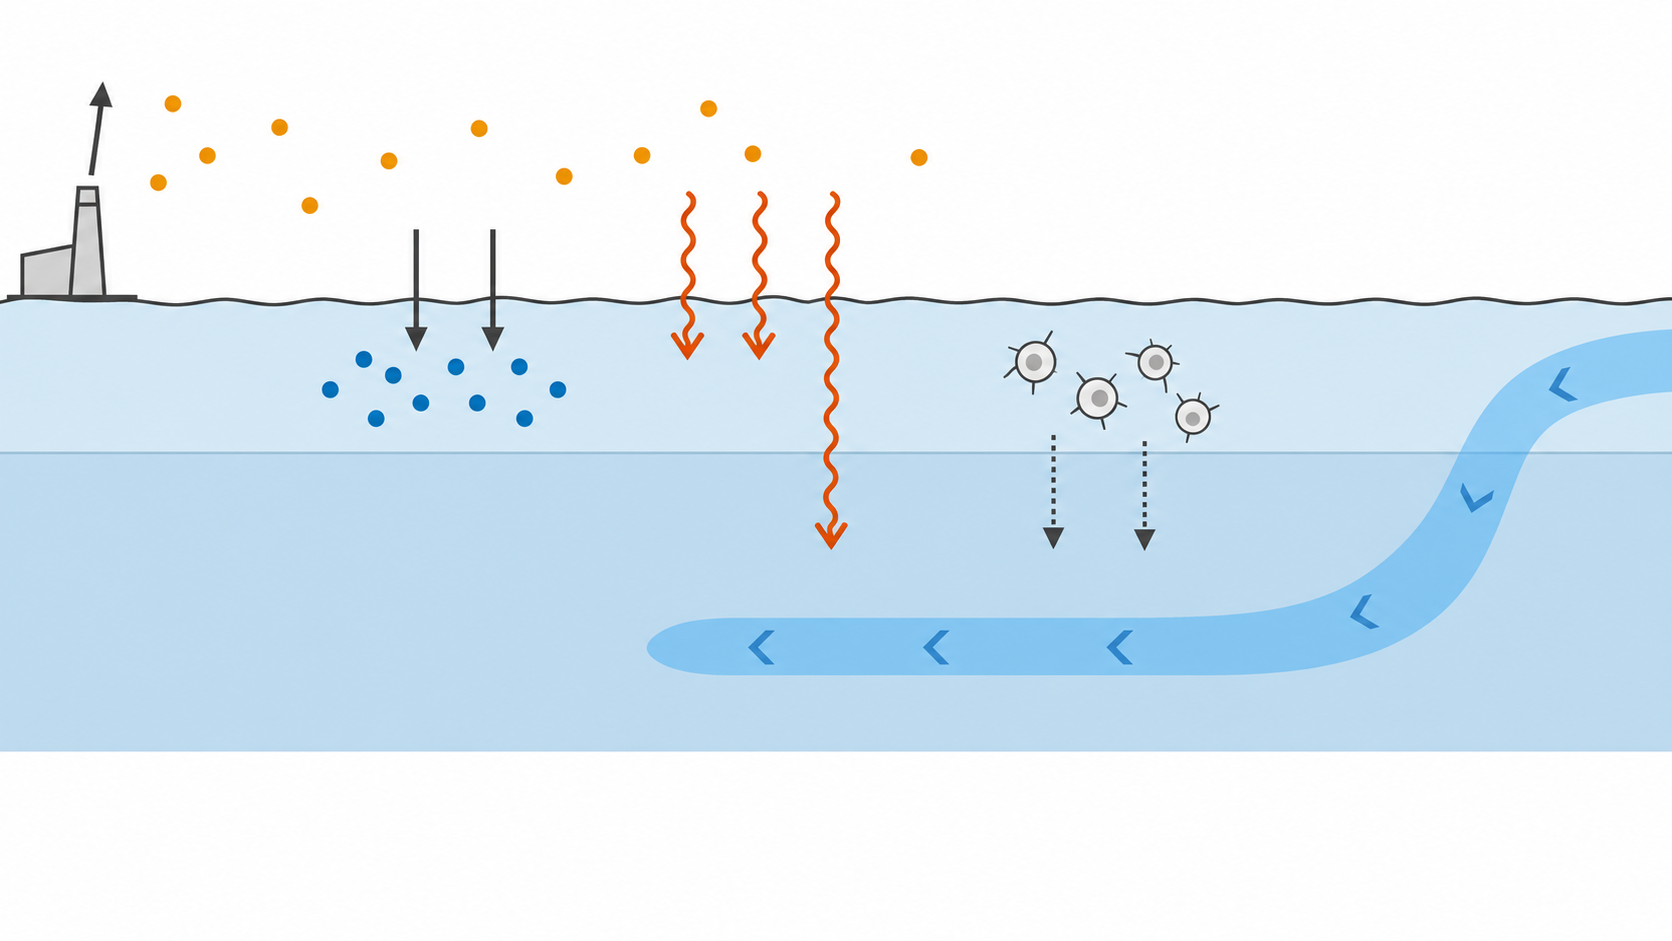
\includegraphics[width=\linewidth]{figures/ch04/ch04-04b-schematic-base.png}};
\begin{scope}[x={(img.south east)},y={(img.north west)},font=\sffamily\small]
  \node at (0.92,0.90) {Atmosphere};
  \node at (0.92,0.66) {Mixed layer};
  \node at (0.92,0.35) {Ocean interior};
  \node[align=left] at (0.06,0.93) {Anthropogenic emissions};
  \node at (0.30,0.88) {CO\textsubscript{2}};
  \node at (0.33,0.70) {Air--sea gas exchange};
  \node at (0.30,0.60) {Dissolved inorganic carbon};
  \node at (0.55,0.70) {Heat uptake};
  \node[align=center] at (0.80,0.45) {Sinking and transport\\of water};
  \node at (0.48,0.62) {Phytoplankton};
  \node[align=center] at (0.48,0.42) {Sinking particles\\(biological pump)};
  \node[align=center,font=\scriptsize] at (0.50,0.04) {%
    Legend: carbon flux / heat flux / water transport / sinking particles};
\end{scope}
\end{tikzpicture}
}}
\end{minipage}
\caption{The schematic follows the same visual language as the data figures. Left (deliberately inconsistent): glossy 3D rendering, a decorative sun and ship, unrequested whales and fish added by the model, and single-colour arrows standing for multiple processes. Right: redrawn to the specification using a text-free base image with TikZ overlay labels; semantic colour is reserved for atmospheric $\text{CO}_2$ (orange), seawater dissolved inorganic carbon (blue), heat (vermilion), and water transport (sky blue), with a distinct arrow shape for each process. Both are model-generated schematics, not to scale.}\label{fig:ch04-04}
\end{figure}

Notice also how the right panel of Figure~\ref{fig:ch04-04} respects the scientific boundary of the \textbf{biological pump}. Phytoplankton fix carbon and export sinking particulate organic carbon to the deep ocean (dotted arrows), but this biological pump mainly cycles \textit{natural} carbon; net oceanic uptake of \textbf{anthropogenic $\text{CO}_2$} since industrialization is governed primarily by air--sea gas exchange, carbonate buffer chemistry, and physical circulation (Sabine et al., 2004; Gruber et al., 2019; Fox-Kemper et al., 2023; Canadell et al., 2023). The right panel therefore places the main anthropogenic uptake pathway (left-middle straight dark-gray arrows $\rightarrow$ blue DIC dots $\rightarrow$ right-hand sky-blue sinking water band) separately from the phytoplankton cells and thinner dotted export arrows in the middle-right, avoiding the visual misconception that phytoplankton directly pump anthropogenic $\text{CO}_2$ into the deep ocean.

\section{Constrain with Prompts, Then Check Every Item}

Enforcing a visual specification with AI tools requires recognizing two practical realities. First, \textbf{conversational AI assistants do not know subfield conventions and may recommend retracted papers when asked to justify a figure design}---for instance, a high-profile 2018 \textit{Nature} paper estimating ocean heat uptake from atmospheric $\text{O}_2$ and $\text{CO}_2$ (Resplandy et al., 2018) was retracted in 2019 over uncertainty and trend-method errors. Every reference must be checked for retraction status via Crossref. Second, \textbf{\scidraw{} currently has no project-level or cross-session style memory}, and interface style presets are no substitute for your manuscript specification.

The reliable workflow is to save your one-page specification as a versioned document (Figure~\ref{fig:ch04-02}), distil it into two copy-ready \textbf{style blocks}, paste the relevant block at the start of every new session, and verify each rendered figure item by item. The core clauses of our specification (v1) are summarized below:

\begin{BookNote}
\textbf{Core Clauses of the One-Page Visual Specification (v1):}
\begin{itemize}
\item \textbf{A.\ Semantic colours (Okabe--Ito base):} Atmospheric carbon \texttt{\#E69F00} (orange: Fig.\ 2a, Fig.\ 4a atmospheric growth, Fig.\ 1 atmospheric $\text{CO}_2$ dots; never for heat or ocean variables); ocean carbon \texttt{\#0072B2} (blue: Fig.\ 2b seawater $p\text{CO}_2$, Fig.\ 4 ocean sink and share, Fig.\ 1 DIC dots; never for water background or heat); land carbon \texttt{\#009E73} (bluish green: Fig.\ 4a land sink only; never for phytoplankton icons); heat \texttt{\#D55E00} (vermilion: Fig.\ 3 depth curves and Fig.\ 1 heat arrows; never for carbon); seawater pH \texttt{\#CC79A7} (reddish purple: Fig.\ 2c only); anthropogenic emissions \texttt{\#3C3C3C} (dark gray); water transport \texttt{\#56B4E9} (sky blue: Fig.\ 1 circulation band only); neutral grays \texttt{\#F2F2F2}, \texttt{\#BDBDBD}, \texttt{\#7A7A7A} (backgrounds, icon fills, reference lines).
\item \textbf{B.\ Type hierarchy at final size:} Width $174\ \text{mm}$ (double column) for Figs.\ 1, 2, 4; $85\ \text{mm}$ (single column) for Fig.\ 3. Panel letters $8\ \text{pt}$ bold lowercase \textbf{a}, \textbf{b}, \textbf{c} (top-left outside axes); axis labels $7\ \text{pt}$ regular; ticks and direct curve labels $6\ \text{pt}$ regular (direct labels match series colour); schematic overlay labels $7\ \text{pt}$ (objects) and $6\ \text{pt}$ (processes). No internal figure titles; parenthetical SI units ($10^{22}\ \text{J}$, $\text{GtC yr}^{-1}$, $\mu\text{atm}$, ppm).
\item \textbf{C--E.\ Lines, arrows, and icons:} Follow Tables~\ref{tab:ch04-lines} and \ref{tab:ch04-arrows}. Icons use $0.75\ \text{pt}$ \texttt{\#3C3C3C} rounded outlines and neutral gray fills, with no gradients, shadows, or 3D effects; exclude sun, ships, icebergs, whales, and fish.
\item \textbf{F.\ Layout and export:} Keep only left and bottom axes ($0.6\ \text{pt}$, outward ticks), no grids, direct labels instead of legend boxes, $4\ \text{mm}$ panel gap; export vector PDF and high-resolution PNG with identical geometry across language editions.
\end{itemize}
\end{BookNote}

At the start of each new data-plotting session in \scidraw{} Scientific Visualization (\sdtool{sci-vis}), paste this data-figure style block:

\begin{Prompt}
Apply this paper-wide figure style exactly (visual spec v1):
- Colours by meaning, no other hues: atmospheric CO2 #E69F00; ocean carbon
  #0072B2; land carbon #009E73; heat #D55E00; seawater pH #CC79A7;
  emissions #3C3C3C; neutral grays #7A7A7A and #BDBDBD only.
- Monthly values: 0.5 pt line in a 50% lighter tint of the series colour.
  Deseasonalized or smoothed values: 1.2 pt solid line. Discrete cruise samples:
  small dots, no connecting line. Uncertainty: band in the series colour at 20%
  opacity, no edge line. Reference lines: 0.5 pt dashed #7A7A7A.
- Sans-serif font. Axis labels 7 pt, tick labels 6 pt, panel letters 8 pt bold
  lowercase (a, b, c) outside the top-left of each axes.
- No title inside the figure, no grid, no legend box: label each series
  directly at its right end in the series colour.
- Only left and bottom axes, 0.6 pt, ticks pointing outward.
- Final size 174 mm wide x 60 mm high.
Keep every data value unchanged: do not smooth, resample, interpolate or drop
rows unless I ask.
\end{Prompt}

When generating a schematic in AI Drawing (\sdtool{ai-drawing}) or via the Mechanism Figure Generator (\sdtool{mechanism-figure-generator}), paste the schematic style block:

\begin{Prompt}
Flat 2D scientific schematic of ocean heat and carbon uptake, landscape 16:9,
pure white background. ABSOLUTELY NO TEXT: no letters, no words, no numbers, no
symbols, no labels, no legend, no title.
STYLE (paper-wide visual spec v1): flat vector illustration; all outlines 0.75 pt
dark gray #3C3C3C with rounded joins; no gradients, no shadows, no highlights,
no 3D, no glow, no texture, no realistic water. Icons use neutral fills only
(#F2F2F2, #BDBDBD). Colour is used ONLY for the following quantities:
orange #E69F00 = CO2 in the atmosphere; blue #0072B2 = dissolved inorganic
carbon in seawater; vermilion #D55E00 = heat; sky blue #56B4E9 = water
transport. Nothing else may use these colours.
REGIONS (top to bottom): Top 25% atmosphere, white; thin dark gray gently wavy
line at 25% height (sea surface); 25-45% surface mixed layer (#DCEBF5); 45-90%
ocean interior (#C9DEEE); bottom 10% empty white reserved for a legend.
DO NOT DRAW: sun, rays, clouds, ships, fish, ice, land masses other than the
short ground line, sea floor details, coral, bubbles, any charts or data.
\end{Prompt}

Keep two precautions in mind when using \sdtool{sci-vis}. First, upload integrity checks (verifying file hashes, byte counts, and row counts) confirm only that the input file was not truncated, not that units, pH scales, anomaly baselines, or colours are scientifically valid. Second, multi-turn conversational edits often trigger \textbf{style drift}: asking to ``add a thin vertical dashed line at December 2022'' can cause regenerated code to quietly revert tick font sizes to library defaults or reintroduce a legend box. Re-verify colours, font sizes, and line styles after every edit, use version history to roll back when drift occurs, and run the Figure Checker (\sdtool{figure-checker}) to screen resolution, grayscale contrast, and colour-vision risk before final export.

\section{Case Study: Turning Four Standalone Figures into One Cohesive Set}

We now follow Maya's four figures from data inventory and specification drafting through redrawing and cross-figure verification.

\textbf{Step 1: Inventory the raw datasets and quality-control rules.} Four public datasets were downloaded on 29 October 2026 (Table~\ref{tab:ch04-sources}). In Figure 2, Mauna Loa atmospheric $\text{CO}_2$ is a \textbf{dry-air mole fraction} ($\text{ppm}$), whereas Station ALOHA surface seawater $p\text{CO}_2$ is an \textbf{in situ partial pressure} ($\mu\text{atm}$) calculated from DIC and total alkalinity. Because the two quantities have different physical dimensions despite sharing numerical values near $300\text{--}430$, they are plotted in separate side-by-side panels (\textbf{a}, \textbf{b}, \textbf{c}) rather than on a single axis.

\begin{table}[htbp]\centering\scriptsize
\setlength{\tabcolsep}{2.5pt}
\renewcommand{\arraystretch}{1.12}
\caption{Public datasets, quality-control rules, and attribution requirements for the four case-study figures (downloaded 29 October 2026).}\label{tab:ch04-sources}
\begin{tabularx}{\linewidth}{@{}>{\raggedright\arraybackslash}p{20mm}>{\raggedright\arraybackslash}p{24mm}>{\raggedright\arraybackslash}p{18mm}Y>{\raggedright\arraybackslash}p{26mm}@{}}
\toprule
\textbf{Dataset (Figure)} & \textbf{File and size} & \textbf{Fields and units} & \textbf{Data processing and QC assertions} & \textbf{Licence and attribution} \\
\midrule
Mauna Loa atmospheric $\text{CO}_2$ (Fig.\ 2a) & \path{co2_mm_mlo.csv}; 823 rows (1958-03 to 2026-09) & \texttt{average}, \path{deseasonalized} ($\text{ppm}$) & Skip \texttt{\#} header lines; assert zero $-99.99$ missing values (mean $361.44\ \text{ppm}$); apply no extra smoothing; mark the Dec 2022--Jul 2023 Mauna Loa eruption relocation to Maunakea & U.S.\ federal government public data; credit both NOAA GML and Scripps (Keeling) \\
HOT Station ALOHA carbonate system (Fig.\ 2b, c) & \path{HOT_surface_CO2.txt}; 355 rows (from 1988-10-31) & \path{pCO2calc_insitu} ($\mu\text{atm}$), \path{pHcalc_insitu} & Skip 8-line header; replace values $\le -900$ (missing code $-999$) with \texttt{NaN}, leaving 346 valid cruises; parse two-digit years into 1988--2026; verify pH scale in \path{HOT_surface_CO2_readme.pdf} for caption & Cite Dore et al.\ (2009) per file header; no explicit open licence stated, so redrawing requires strict citation \\
Global ocean heat content anomaly (Fig.\ 3) & \path{pent_h22-w0-700m.dat} and \texttt{2000m.dat}; 67 rows each & \texttt{YEAR} (1957.5--2023.5), \texttt{WO}, \texttt{WOse} ($10^{22}\ \text{J}$) & Assert identical midpoint years and row counts across both depth files (means $3.84$ and $5.09\times 10^{22}\ \text{J}$); shade $\text{WO} \pm 1\ \text{WOse}$; confirm climatological baseline period in NCEI documentation & NOAA NCEI U.S.\ government work; cite Levitus et al.\ (2012) \\
Global Carbon Budget 2025 (Fig.\ 4) & \path{GlobalCarbonBudget_v2025.xlsx}; 66 rows (1959--2024) & Emissions and three sinks ($\text{GtC yr}^{-1}$) & Read sheet \texttt{Global Carbon Budget} (header row 22); total emissions = fossil + land-use change; shade mean uncertainties ($\pm 0.4$ ocean, $\pm 0.5$ land); compute ocean share (mean $27.01\%$) and 10-yr centred running mean in panel b & Fair Use Statement; cite Friedlingstein et al.\ (2026) and acknowledge Global Carbon Project \\
\bottomrule
\end{tabularx}
\end{table}

\textbf{Step 2: Redraw the conceptual schematic (Fig.\ 1) and audit generative deviations.} Compare the prompt used for the inconsistent 3D schematic on the left of Figure~\ref{fig:ch04-04}:

\begin{Prompt}
A glossy, highly polished 3D illustration of an ocean cross-section for a
climate science paper, landscape 16:9. Photorealistic blue waves on top, a
bright sun with radiating rays in a gradient orange-to-blue sky, a small ship
on the surface, shiny glass-like water with caustics and depth of field.
Thick glowing red 3D arrows go from the sky into the water and also from a
factory into the sky; thick glowing blue 3D arrows curve through the water and
also go from the air into the water. Dramatic lighting, lens flare, strong
shadows, saturated colors. No text, no letters, no numbers, no labels.
\end{Prompt}

Requesting ``glossy 3D'', ``photorealistic blue waves'', and ``dramatic lighting'' while assigning red and blue arrows to multiple processes directly caused the visual conflicts in Table~\ref{tab:ch04-diag}---and without an exclusion list, the model added a whale, fish schools, and reefs.

To redraw the right panel of Figure~\ref{fig:ch04-04}, we appended the following seven object and process instructions to the schematic style block from Section 4.5 (full prompt in the \texttt{cases/} directory of the book repository):

\begin{Prompt}
OBJECTS AND PROCESSES (draw exactly these, nothing else):
1. Top-left: one simple factory chimney icon in neutral gray on a short ground
   line, with one straight dark gray arrow (filled head) rising into the air.
2. Atmosphere: about 12 small orange dots scattered in the left and middle.
3. Air-sea gas exchange: two straight dark gray arrows with filled heads, going
   down from the atmosphere through the sea surface into the mixed layer.
4. Mixed layer: about 10 small blue #0072B2 dots near the two arrows.
5. Heat uptake: three vermilion wavy arrows with open V-shaped heads, going down
   into the mixed layer; the rightmost continues into the ocean interior.
6. Water transport: on the right, one broad semi-transparent sky-blue band from
   the mixed layer curving down into the interior and running leftward, with
   chevron marks pointing along the flow.
7. Biological pump: 3-4 small round phytoplankton cell icons (neutral fill, gray
   outline) in the mixed layer, and two dotted dark gray arrows pointing down.
Leave white space around each process for labels.
\end{Prompt}

Generating three candidates from this prompt and auditing each image reveals how generative outputs behave in practice:
\begin{itemize}
\item \textbf{Candidate 1 (rejected for contradictory flow direction):} All major objects appeared, but inside the sky-blue transport band on the right, upper and middle chevrons pointed up-right while bottom chevrons pointed left, making the flow collide head-on with itself.
\item \textbf{Candidate 2 (selected for Figure~\ref{fig:ch04-04}, right):} All seven object groups and four arrow types were present, chevrons inside the transport band pointed consistently down-left and leftward along the flow, and no text or forbidden decorative objects appeared.
\item \textbf{Candidate 3 (rejected):} Flow direction was consistent, but the model added unrequested spine-like protrusions to the phytoplankton cells, thickened the dotted arrows, and yielded a slightly lower luminance contrast for the vermilion heat arrows against the interior background under simulated deuteranomaly ($2.17:1$ vs.\ $2.36:1$ in Candidate 2).
\end{itemize}

A pixel audit of the selected Candidate 2 base image still uncovers three real deviations: (1) \textbf{approximate hex colours}---median RGB values across object regions measured \texttt{\#ED9106} for atmospheric orange dots (spec \texttt{\#E69F00}), \texttt{\#0571BA} for seawater blue dots (spec \texttt{\#0072B2}), \texttt{\#DD4E0A} for vermilion heat arrows (spec \texttt{\#D55E00}), and \texttt{\#3F3F40} for dark-gray carbon arrows (spec \texttt{\#3C3C3C}), with zero pixels matching the exact target hex strings and slight shading across the water layers and smokestack; (2) \textbf{shifted layer proportions and object placement}---the sea surface, mixed-layer base, and bottom legend margin fell at roughly $32\%$, $48\%$, and $80\%$ of height rather than $25\%$, $45\%$, and $90\%$, and the four phytoplankton cells sat in the middle-right of the mixed layer, so the overlaid ``Phytoplankton'' label placed at the preset centre coordinate landed in open water to their left (Figure~\ref{fig:ch04-04}, right) and requires a rightward nudge in TikZ; and (3) \textbf{native resolution limits}---at $174\ \text{mm}$ width, the $1672 \times 941\ \text{px}$ raster image provides $244\ \text{ppi}$ with no editable vector stroke weights.

\textbf{Step 3: Redraw the three data figures (Figs.\ 2--4) to the specification.} Importing all style constants from a shared module produced Figures~\ref{fig:ch04-05}--\ref{fig:ch04-07} (Table~\ref{tab:ch04-revisions}).

\begin{figure}[htbp]\centering
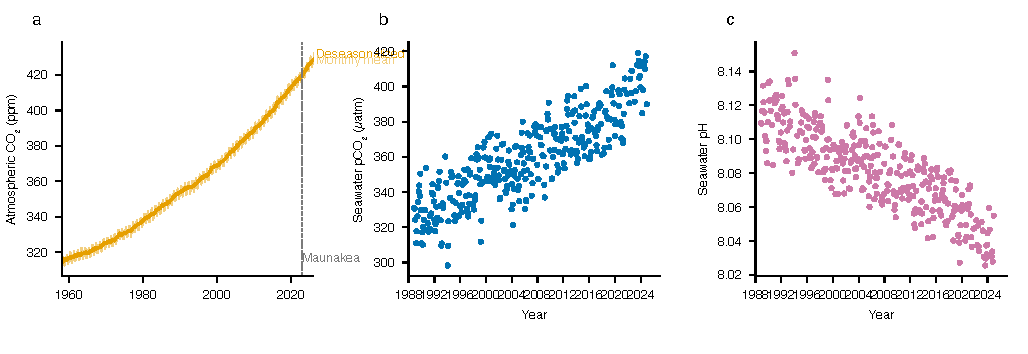
\includegraphics[width=\linewidth]{figures/ch04/ch04-05-fig2-carbonate-en.pdf}
\caption{Paper Fig.\ 2 redrawn to the specification: atmospheric $\text{CO}_2$ and the surface seawater carbonate system in the subtropical North Pacific. (a) Monthly mean (thin light-orange line) and deseasonalized (thick orange line) atmospheric $\text{CO}_2$ at Mauna Loa Observatory; March 1958--April 1974 data are from Scripps, and December 2022--July 2023 observations were made at Maunakea after the Mauna Loa eruption (gray dashed line). (b) Surface seawater $p\text{CO}_2$ at Station ALOHA (HOT), calculated in situ from DIC and total alkalinity; one dot per cruise. (c) Surface seawater pH at the same station (calculated at in situ temperature; pH scale to be confirmed). Data: NOAA GML and Scripps; HOT (Dore et al., 2009), downloaded 29 October 2026.}\label{fig:ch04-05}
\end{figure}

In Figure~\ref{fig:ch04-05} (Paper Fig.\ 2), panel \textbf{a} plots Mauna Loa $\text{CO}_2$ in semantic orange (\texttt{\#E69F00}) with the Maunakea relocation dashed line; panel \textbf{b} plots 346 valid cruises of surface seawater $p\text{CO}_2$ as unlinked ocean-carbon blue dots (\texttt{\#0072B2}); and panel \textbf{c} plots surface pH in reddish purple (\texttt{\#CC79A7}). Checking at $100\%$ print size catches three remaining layout details: at the top right of panel \textbf{a}, ``Deseasonalized'' and ``Monthly mean'' overlap vertically and collide with the ``420'' y-tick label of panel \textbf{b}; in panels \textbf{b} and \textbf{c}, the 4-year x-tick labels crowd together and should be widened to 10-year intervals; and the dropped subscript ``2'' in the y-axis labels of panels \textbf{a} and \textbf{b} needs explicit math-mode subscripting.

\begin{figure}[htbp]\centering
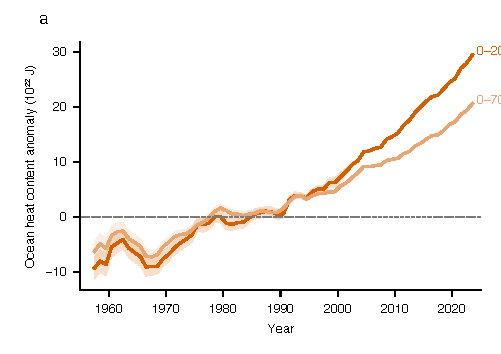
\includegraphics[width=0.58\linewidth]{figures/ch04/ch04-06-fig3-ohc-en.pdf}
\caption{Paper Fig.\ 3 redrawn to the specification: global ocean heat content anomaly. Pentadal heat content anomalies for $0\text{--}700\ \text{m}$ (light vermilion) and $0\text{--}2000\ \text{m}$ (dark vermilion), in $10^{22}\ \text{J}$, plotted at five-year window midpoints; shading shows $\pm 1$ standard error from NCEI, and the dashed line marks zero. The climatological baseline period must be confirmed in NCEI documentation. Data: NOAA NCEI (method of Levitus et al., 2012, and updates).}\label{fig:ch04-06}
\end{figure}

In Figure~\ref{fig:ch04-06} (Paper Fig.\ 3, single-column width $85\ \text{mm}$), both curves use the vermilion heat hue (\texttt{\#D55E00}) separated by lightness, with $\pm 1\ \text{WOse}$ bands and a dashed zero line showing sustained ocean heat uptake (von Schuckmann et al., 2023). Inspecting the right edge shows that ``$0\text{--}2000\ \text{m}$'' and ``$0\text{--}700\ \text{m}$'' are clipped to ``\texttt{0--20}'' and ``\texttt{0--70}'', demonstrating that direct right-end labels require widening the right margin or upper x-axis limit.

\begin{figure}[htbp]\centering
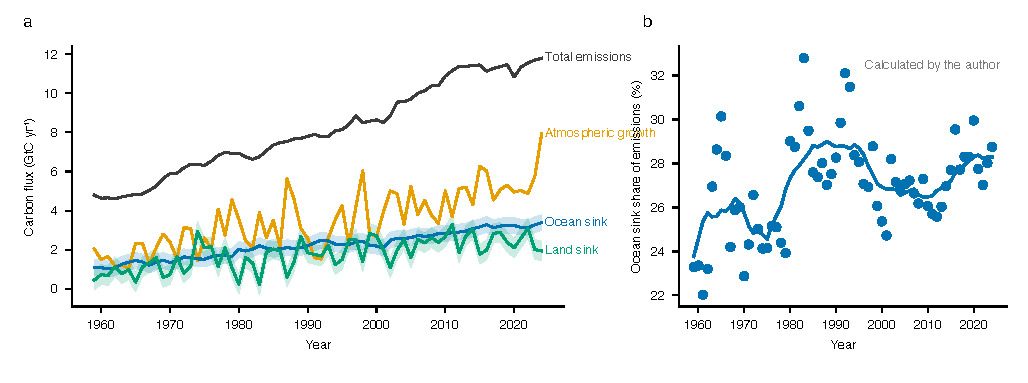
\includegraphics[width=\linewidth]{figures/ch04/ch04-07-fig4-budget-en.pdf}
\caption{Paper Fig.\ 4 redrawn to the specification: partitioning of anthropogenic $\text{CO}_2$ emissions. (a) Combined fossil and land-use change emissions (dark gray) with atmospheric growth (orange), ocean sink (blue), and land sink (bluish green), in $\text{GtC yr}^{-1}$; bands show mean GCB uncertainties ($\pm 0.4$ ocean, $\pm 0.5\ \text{GtC yr}^{-1}$ land). (b) Ocean sink share of total emissions, calculated by the author from GCB 2025 data (dots, annual values; curve, 10-year centred running mean). Budget imbalance and cement carbonation sink are omitted. Data: Global Carbon Budget 2025 (Friedlingstein et al., 2026).}\label{fig:ch04-07}
\end{figure}

In Figure~\ref{fig:ch04-07} (Paper Fig.\ 4), panel \textbf{a} replaces the rainbow stacked area plot with four semantic curves and uncertainty bands, while panel \textbf{b} plots the author-computed ocean sink share (mean $27.01\%$) as blue annual dots and a 10-year running mean marked ``Calculated by the author''. At $100\%$ zoom, ``Atmospheric growth'' slightly grazes the left spine of panel \textbf{b}, and the y-axis unit requires an explicit minus sign ($\text{GtC yr}^{-1}$).

\begin{table}[htbp]\centering\footnotesize
\setlength{\tabcolsep}{3pt}
\renewcommand{\arraystretch}{1.15}
\caption{Revision log from the inconsistent draft (Figure~\ref{fig:ch04-01}) to the redrawn figures (Figures~\ref{fig:ch04-04}--\ref{fig:ch04-07}).}\label{tab:ch04-revisions}
\begin{tabularx}{\linewidth}{@{}>{\raggedright\arraybackslash}p{14mm}Y>{\raggedright\arraybackslash}p{20mm}>{\raggedright\arraybackslash}p{36mm}@{}}
\toprule
\textbf{Figure} & \textbf{Specific revisions applied} & \textbf{Clause} & \textbf{Verification and audit notes} \\
\midrule
Fig.\ 1 & Removed 3D gloss, sun, ship, whale, and fish; generated flat 2D base; redrew four process arrows per Table~\ref{tab:ch04-arrows}; added TikZ labels & Clauses A, D, E & Rejected Candidate 1 (flow collision), chose Candidate 2; noted approximate hex values and rightward phytoplankton offset \\
Fig.\ 2a & Changed dual red lines to orange \texttt{\#E69F00} ($0.5\ \text{pt}$ light monthly + $1.2\ \text{pt}$ deseasonalized); added Maunakea dashed line & Clauses A, C & Eyedropper hex check; caught end-label overlap and collision with panel b y-ticks \\
Fig.\ 2b, c & Changed connected green/blue lines to unlinked $2.5\ \text{pt}$ dots in \texttt{\#0072B2} (ocean carbon) and \texttt{\#CC79A7} (pH) & Clauses A, C & Verified 346 valid cruises unlinked; noted crowded 4-yr x-ticks to widen to 10-yr spacing \\
Fig.\ 3 & Replaced red/green lines with two lightnesses of vermilion (\texttt{\#D55E00}); added $\pm 1\ \text{WOse}$ bands and zero line; fixed \texttt{1e23} offset & Clauses A, B, C & Separable under deuteranomaly simulation (Figure~\ref{fig:ch04-03}); right-end labels clipped, need wider right margin \\
Fig.\ 4 & Replaced \texttt{jet} stacked areas with four semantic curves + bands; added panel b ocean share marked ``Calculated by the author'' & Clauses A, B, C & Verified 66-yr values against workbook; ``Atmospheric growth'' label grazes panel b spine \\
All four & Unified sans-serif font and 8/7/6 pt hierarchy; bold lowercase \textbf{a}--\textbf{c}; removed internal titles, grids, and legend boxes & Clauses B, F & Measured point sizes in $100\%$ PDF; caught silent dropout of Unicode subscript 2 and superscript minus \\
\bottomrule
\end{tabularx}
\end{table}

\textbf{Step 4: Side-by-side contact-sheet comparison, finalized captions, and verification log.} Assembling the four revised figures into the same $2 \times 2$ layout as Figure~\ref{fig:ch04-01} with a bottom semantic colour bar yields Figure~\ref{fig:ch04-08}.

\begin{figure}[htbp]\centering
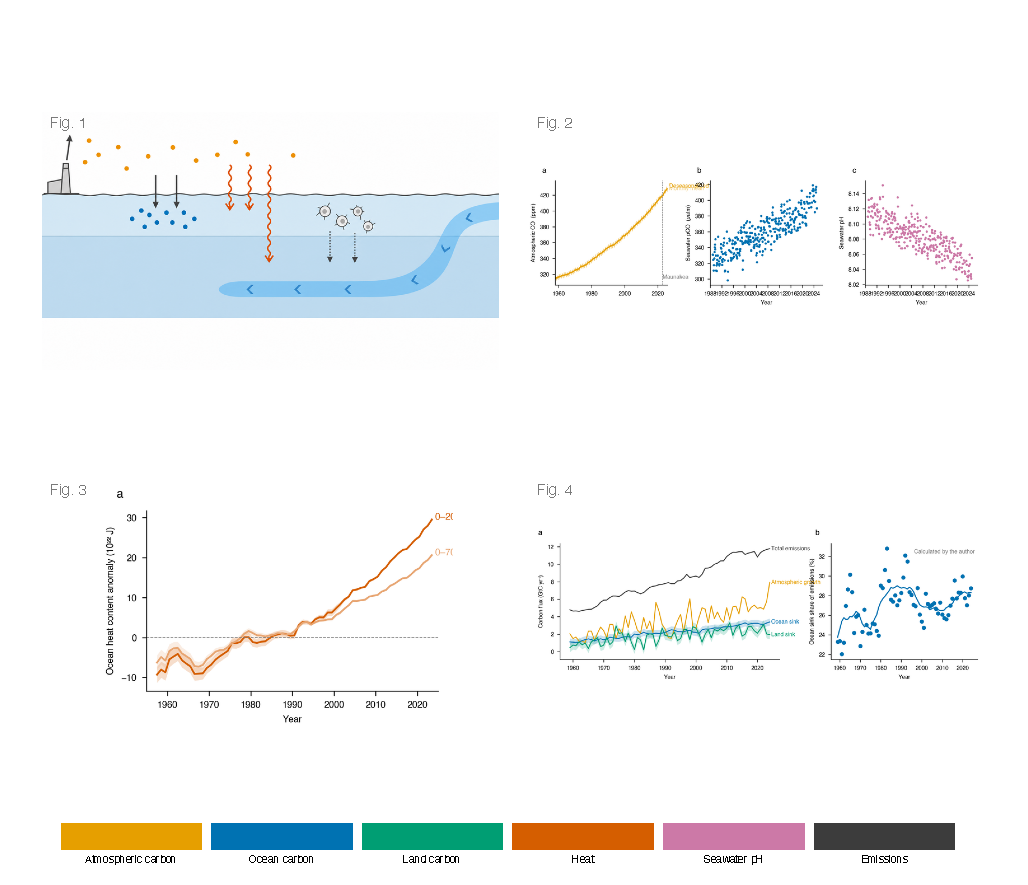
\includegraphics[width=\linewidth]{figures/ch04/ch04-08-consistent-set-en.pdf}
\caption{The four manuscript figures after applying the one-page visual specification. Every semantic colour carries a single meaning across the paper (bottom strip), and fonts, sizes, panel letters, line styles, and arrow shapes are unified. Compared with Figure~\ref{fig:ch04-01}, the underlying data are identical; only the visual language has changed.}\label{fig:ch04-08}
\end{figure}

Comparing Figure~\ref{fig:ch04-08} with Figure~\ref{fig:ch04-01}, readers can trace orange (atmospheric carbon) directly across Fig.\ 1, Fig.\ 2a, and Fig.\ 4a; trace blue (ocean carbon) across Fig.\ 1, Fig.\ 2b, and Fig.\ 4a, b; and trace vermilion (heat) from Fig.\ 1 to Fig.\ 3 without consulting a legend box. The finalized caption for Paper Fig.\ 1 is given below, followed by the cross-figure verification log (Table~\ref{tab:ch04-verify}).

\begin{BookNote}
\textbf{Finalized Caption for Paper Figure 1:} \textbf{Figure 1 | Main pathways of ocean heat and anthropogenic $\text{CO}_2$ uptake.} Excess heat enters the surface mixed layer across the air--sea interface (wavy arrows) and is carried into the ocean interior by mixing and the sinking of water masses (pale-blue band). Anthropogenic $\text{CO}_2$ dissolves into surface seawater by air--sea gas exchange (straight arrows), raising seawater $p\text{CO}_2$ and lowering pH, and is likewise transported into the interior. Phytoplankton fix carbon that is exported as sinking particles (dotted arrows); this biological pump mainly moves carbon of the natural cycle, whereas uptake of anthropogenic $\text{CO}_2$ is governed chiefly by gas exchange, seawater chemistry, and circulation. Schematic, not to scale; regional and seasonal variations, sea ice, sediments, and river inputs are omitted. Compiled from Sabine et al.\ (2004), Gruber et al.\ (2019), and IPCC AR6 WGI Chapters 5 and 9 (Canadell et al., 2023; Fox-Kemper et al., 2023).
\end{BookNote}

\begin{table}[htbp]\centering\footnotesize
\setlength{\tabcolsep}{3pt}
\renewcommand{\arraystretch}{1.15}
\caption{Cross-figure verification log for the four case-study manuscript figures.}\label{tab:ch04-verify}
\begin{tabularx}{\linewidth}{@{}>{\raggedright\arraybackslash}p{38mm}YYYY@{}}
\toprule
\textbf{Verification item} & \textbf{Fig.\ 1} & \textbf{Fig.\ 2} & \textbf{Fig.\ 3} & \textbf{Fig.\ 4} \\
\midrule
Semantic colours match Clause A across figures & Pass (hex approximate) & Pass & Pass & Pass \\
Separable under CVD simulation and in grayscale & Separable via arrow shapes & Separate panels, no conflict & Pass (Figure~\ref{fig:ch04-03}) & Pass (with direct labels) \\
Type sizes match 8/7/6 pt at $100\%$ print size & Pass & Pass & Pass & Pass \\
Panel letters and units consistent, no glyph dropout or clipping & Nudge ``Phytoplankton'' label right & Fix subscript 2, label overlap, 4-yr ticks & Widen right margin for clipped labels & Fix minus sign in $\text{yr}^{-1}$ and label margin \\
Lines and arrows match Tables~\ref{tab:ch04-lines} and \ref{tab:ch04-arrows} & Pass & Pass & Pass & Pass \\
Years and row counts match raw files & Not applicable & 823 rows / 346 cruises & 67 rows (both depths) & 66 rows (1959--2024) \\
Author calculations and uncertainties in caption & Not applicable & Confirm pH scale in readme & Confirm baseline in NCEI docs & Marked ``Calculated by the author'' \\
Citations complete and domain review scheduled & Pending oceanographer review & NOAA GML, Scripps, HOT cited & NOAA NCEI, Levitus cited & GCB 2025, GCP cited \\
\bottomrule
\end{tabularx}
\end{table}

\section{What AI Can and Cannot Do in This Step}

Table~\ref{tab:ch04-01} summarizes the division of responsibilities between AI tools and the author when establishing a paper-wide visual language.

\begin{table}[htbp]\centering\scriptsize
\setlength{\tabcolsep}{3pt}
\renewcommand{\arraystretch}{1.12}
\caption{What AI can do, what it cannot reliably do, and what the author must verify when building a paper-wide visual language.}\label{tab:ch04-01}
\begin{tabularx}{\linewidth}{@{}>{\raggedright\arraybackslash}p{19mm}YYY@{}}
\toprule
\textbf{Step} & \textbf{What AI can do} & \textbf{What AI cannot do / where it fails} & \textbf{What the author must verify} \\
\midrule
Drafting the specification & Conversational AI can propose an initial semantic colour table and type hierarchy from your figure list and suggest accessible palettes & Does not know your subfield's colour conventions or journal dimensions; may cite non-existent or retracted papers as justification & Check every clause against domain norms and journal guidelines; verify all DOIs and retraction statuses via Crossref \\
Cross-figure memory & --- & \scidraw{} has no project-level style memory and does not remember your specification across sessions or tools & Save the specification as a versioned document; paste the style block into every new session \\
Applying style to data plots & \sdtool{sci-vis} generates plots from a style block, applies conversational edits, and restores earlier versions & Multi-turn edits can trigger style drift (reverting font sizes, restoring legends, or clipping labels); ``done'' does not mean compliant & Sample hex values, measure type at $100\%$ size, check line styles after each turn, and save compliant versions \\
Data integrity checks & \sdtool{sci-vis} checks SHA-256 hashes, byte counts, and row counts of uploaded files & Proves only that no rows were dropped on upload, not that units, pH scales, baselines, or calculations are right & Check start/end dates, row counts, units, and baselines against raw files and documentation \\
Applying style to schematics & Drawing and reference-image editing generate flat schematics with approximate semantic colours & Hex colours, layer ratios, and stroke widths are approximate; may produce conflicting flow chevrons or extra objects & Compare multiple candidates, sample pixel colours, check arrow directions, remove extra objects, and align TikZ labels \\
CVD and technical checks & \sdtool{figure-checker} screens format, resolution, grayscale contrast, and algorithmic CVD risk & Does not audit science; numerical CVD simulation is an approximation and cannot replace human readers & Combine simulation and grayscale checks with review by a reader with CVD; verify science separately \\
Figure captions & \sdtool{figure-legend} drafts caption structure from a rendered figure & Does not know data provenance, processing, or baselines; must never invent them & Supply data sources, download dates, units, uncertainties, and author-calculated items yourself \\
\bottomrule
\end{tabularx}
\end{table}

\section{Chapter Checklist}

\begin{itemize}
\item I have a written one-page visual specification with a version number.
\item Every semantic colour encodes one quantity or reservoir, and every recurring quantity uses the same semantic colour across all figures.
\item Semantic colours do not exceed 6--7 hues; axes, reference lines, backgrounds, and icon bodies use neutral grays.
\item Colours sharing a panel remain distinguishable under colour-vision simulation and in grayscale, or have redundant shape, line-style, or direct-label encoding.
\item Continuous variables use perceptually uniform sequential or diverging colormaps, never rainbow colormaps.
\item Font sizes have been measured at $100\%$ final print size across all four levels (panel letters, axis labels, ticks, annotations).
\item One sans-serif typeface is used throughout, bilingual editions share identical geometry, and subscripts and superscripts have been checked at $200\%$ zoom for missing-glyph boxes or dropped characters.
\item Unit notation and panel letters (\textbf{a}, \textbf{b}, \textbf{c}) follow the same convention in every figure.
\item Every line style and schematic arrow shape has a single meaning, defined once in the legend.
\item Icons use neutral gray fills, match axis stroke weights, and omit unmentioned decorative objects.
\item The style block was pasted into every new session, and colours, font sizes, and margins were re-checked after every conversational edit.
\item Data sources, download dates, processing rules, and author-computed quantities are stated in the captions.
\item I have viewed all figures side by side on a single page at final print size.
\end{itemize}

\section{Exercises}

\begin{enumerate}
\item \textbf{(Pen and paper: Assign semantic colours to your paper)} List all quantities or categories across the figures of a paper you are writing (or a published paper in your field). (a) Group them into no more than six semantic roles; (b) assign each role an Okabe--Ito colour and state ``used for / never used for''; (c) find at least three violations in the existing figures and specify the fix; (d) explain whether your discipline has mandatory colour conventions (such as warm colours for temperature or blue-green for precipitation) and whether your table conflicts with them.
\item \textbf{(Colour-vision and grayscale check)} Pick one data figure from your paper. (a) Export a PNG and check colour-vision risk and grayscale contrast in the \scidraw{} Figure Checker (\sdtool{figure-checker}), or simulate three CVD types using \texttt{colorspacious}; (b) identify the hardest colour pair to distinguish under simulation; (c) resolve the conflict without adding a new hue by using lightness, line style, or direct labels; (d) explain why simulation cannot replace asking a human reader with CVD.
\item \textbf{(Hands-on with \scidraw{}: Constrain a dataset with a style block)} Download \texttt{co2\_mm\_mlo.csv} from NOAA GML, strip \texttt{\#} comment lines, and save a clean CSV (recording its SHA-256 hash and row count). (a) Upload it to \scidraw{} Scientific Visualization (\sdtool{sci-vis}), ask only ``Plot the atmospheric $\text{CO}_2$ time series'', and save the result; (b) open a new session, upload the same file, paste the data-figure style block from Section 4.5, and repeat the request; (c) add two follow-up edits (e.g., ``make the monthly mean line lighter'' and ``add a thin vertical line at December 2022''), checking after each turn whether colours or font sizes drifted; (d) compare versions (a), (b), and (c) in an audit table (colour, font size, line style, labels, row count) and write a one-sentence credit to NOAA GML and Scripps. \textit{(Note: The example figures in this chapter were generated by image models and companion scripts; prompts and generation records are available in the book repository.)}
\end{enumerate}

\section*{References}

{\sloppy
\begin{itemize}
\item Brewer CA. ColorBrewer 2.0: Color advice for cartography. \url{https://colorbrewer2.org}
\item Canadell JG, Monteiro PMS, Costa MH, Cotrim da Cunha L, Cox PM, Eliseev AV, Henson S, Ishii M, Jaccard S, Koven C, Lohila A, Patra PK, Piao S, Rogelj J, Syampungani S, Zaehle S, Zickfeld K. Global carbon and other biogeochemical cycles and feedbacks. In: \textit{Climate Change 2021: The Physical Science Basis. Contribution of Working Group I to the Sixth Assessment Report of the Intergovernmental Panel on Climate Change}. Cambridge University Press; 2023:673--816. doi:10.1017/9781009157896.007
\item Crameri F, Shephard GE, Heron PJ. The misuse of colour in science communication. \textit{Nature Communications}. 2020;11:5444. doi:10.1038/s41467-020-19160-7
\item Dore JE, Lukas R, Sadler DW, Church MJ, Karl DM. Physical and biogeochemical modulation of ocean acidification in the central North Pacific. \textit{Proceedings of the National Academy of Sciences}. 2009;106(30):12235--12240. doi:10.1073/pnas.0906044106
\item Fox-Kemper B, Hewitt HT, Xiao C, A\dh algeirsd\'ottir G, Drijfhout SS, Edwards TL, Golledge NR, Hemer M, Kopp RE, Krinner G, Mix A, Notz D, Nowicki S, Nurhati IS, Ruiz L, Sall\'ee J-B, Slangen ABA, Yu Y. Ocean, cryosphere and sea level change. In: \textit{Climate Change 2021: The Physical Science Basis. Contribution of Working Group I to the Sixth Assessment Report of the Intergovernmental Panel on Climate Change}. Cambridge University Press; 2023:1211--1362. doi:10.1017/9781009157896.011
\item Friedlingstein P, O'Sullivan M, Jones MW, et al. Global Carbon Budget 2025. \textit{Earth System Science Data}. 2026;18:3211--3288. doi:10.5194/essd-18-3211-2026
\item Gruber N, Clement D, Carter BR, Feely RA, van Heuven S, Hoppema M, Ishii M, Key RM, Kozyr A, Lauvset SK, Lo Monaco C, Mathis JT, Murata A, Olsen A, Perez FF, Sabine CL, Tanhua T, Wanninkhof R. The oceanic sink for anthropogenic $\text{CO}_2$ from 1994 to 2007. \textit{Science}. 2019;363(6432):1193--1199. doi:10.1126/science.aau5153
\item Krzywinski M. Elements of visual style. \textit{Nature Methods}. 2013;10(5):371. doi:10.1038/nmeth.2444
\item Levitus S, Antonov JI, Boyer TP, Baranova OK, Garcia HE, Locarnini RA, Mishonov AV, Reagan JR, Seidov D, Yarosh ES, Zweng MM. World ocean heat content and thermosteric sea level change (0--2000 m), 1955--2010. \textit{Geophysical Research Letters}. 2012;39:L10603. doi:10.1029/2012GL051106
\item NOAA Global Monitoring Laboratory. Trends in Atmospheric Carbon Dioxide (Mauna Loa, Hawaii) and Scripps Institution of Oceanography $\text{CO}_2$ Program. \url{https://gml.noaa.gov/ccgg/trends/} and \url{https://scrippsco2.ucsd.edu/}
\item Nu\~nez JR, Anderton CR, Renslow RS. Optimizing colormaps with consideration for color vision deficiency to enable accurate interpretation of scientific data. \textit{PLOS ONE}. 2018;13(8):e0199239. doi:10.1371/journal.pone.0199239
\item Okabe M, Ito K. Color Universal Design (CUD): How to make figures and presentations that are friendly to colorblind people. 2008. \url{https://jfly.uni-koeln.de/color/}
\item Rougier NP, Droettboom M, Bourne PE. Ten simple rules for better figures. \textit{PLoS Computational Biology}. 2014;10(9):e1003833. doi:10.1371/journal.pcbi.1003833
\item Sabine CL, Feely RA, Gruber N, Key RM, Lee K, Bullister JL, Wanninkhof R, Wong CS, Wallace DWR, Tilbrook B, Millero FJ, Peng T-H, Kozyr A, Ono T, Rios AF. The oceanic sink for anthropogenic $\text{CO}_2$. \textit{Science}. 2004;305(5682):367--371. doi:10.1126/science.1097403
\item von Schuckmann K, Mini\`ere A, Gues F, Cuesta-Valero FJ, Kirchengast G, Adusumilli S, Straneo F, et al. Heat stored in the Earth system 1960--2020: where does the energy go? \textit{Earth System Science Data}. 2023;15(4):1675--1709. doi:10.5194/essd-15-1675-2023
\item Wong B. Points of view: Color coding. \textit{Nature Methods}. 2010;7(8):573. doi:10.1038/nmeth0810-573
\item Wong B. Points of view: Typography. \textit{Nature Methods}. 2011;8(4):277. doi:10.1038/nmeth0411-277
\item Wong B. Points of view: Color blindness. \textit{Nature Methods}. 2011;8(6):441. doi:10.1038/nmeth.1618 (Author Correction: \textit{Nature Methods}. 2023;20:1442. doi:10.1038/s41592-023-01974-0)
\end{itemize}
\par}
